\chapter{One-dimensional symmetric phases protected by frieze symmetries}\label{app:frieze}
\section{Synopsis}
In \cref{sec:1Dphases} we reviewed the classification of one-dimensional SPT phases protected by \emph{internal} symmetries acting in an on-site manner. The present project extends this classification to include quasi-one-dimensional \emph{spatial symmetries}. These are encoded in the so-called frieze groups, of which there are seven. We closely follow an approach analogous to that of \cref{sec:1Dphases} and study the action of the symmetry on an injective MPS. We find that these SPT phases are classified by the second cohomology group of the protecting symmetry group over $\rU(1)$, with the additional feature that \emph{orientation-reversing} group elements --- encoding spatial reflection, for instance --- act on $\rU(1)$ via complex conjugation. Additionally, we provide MPS normal forms for each of these phases and explicit renormalisation group fixed-point MPS representations directly in terms of representative cocycles. We also review the SPT classification in the presence of time-reversal symmetry. Finally, we discuss an algorithm that computes cohomology groups of any order and corresponding representative cocycles, including in the presence of non-trivial group action.
%TODO check if newpage is appropriate here
\newpage
\section{Reference}
\textit{One-dimensional symmetric phases protected by frieze symmetries} \par\noindent
\textbf{B. Vancraeynest-De Cuiper}, J. C. Bridgeman, N. Dewolf, J. Haegeman, F. Verstraete \par\noindent
\href{https://doi.org/10.1103/PhysRevB.107.115123}{Physical Review B \textbf{107} (11), 115123 (2023)}, \href{https://doi.org/10.48550/arXiv.2202.12880}{arXiv:2202.12880}
\section{Contributions of the author}
The project underlying this paper grew out of the Master's thesis of Nicolas Dewolf. Therein the classification of SPT phases protected by frieze symmetries was initiated and the framework established. I verified and completed the classification of MPS symmetric under these symmetry groups and their cohomological classification. I have finalised the algorithm based on the Smith normal form for computing group cohomology and cocycles and, conjointly with my supervisors, derived the representative fixed-point matrix product states. The manuscript was mostly written by me.

%\section{One-dimensional symmetric phases protected by frieze symmetries}
%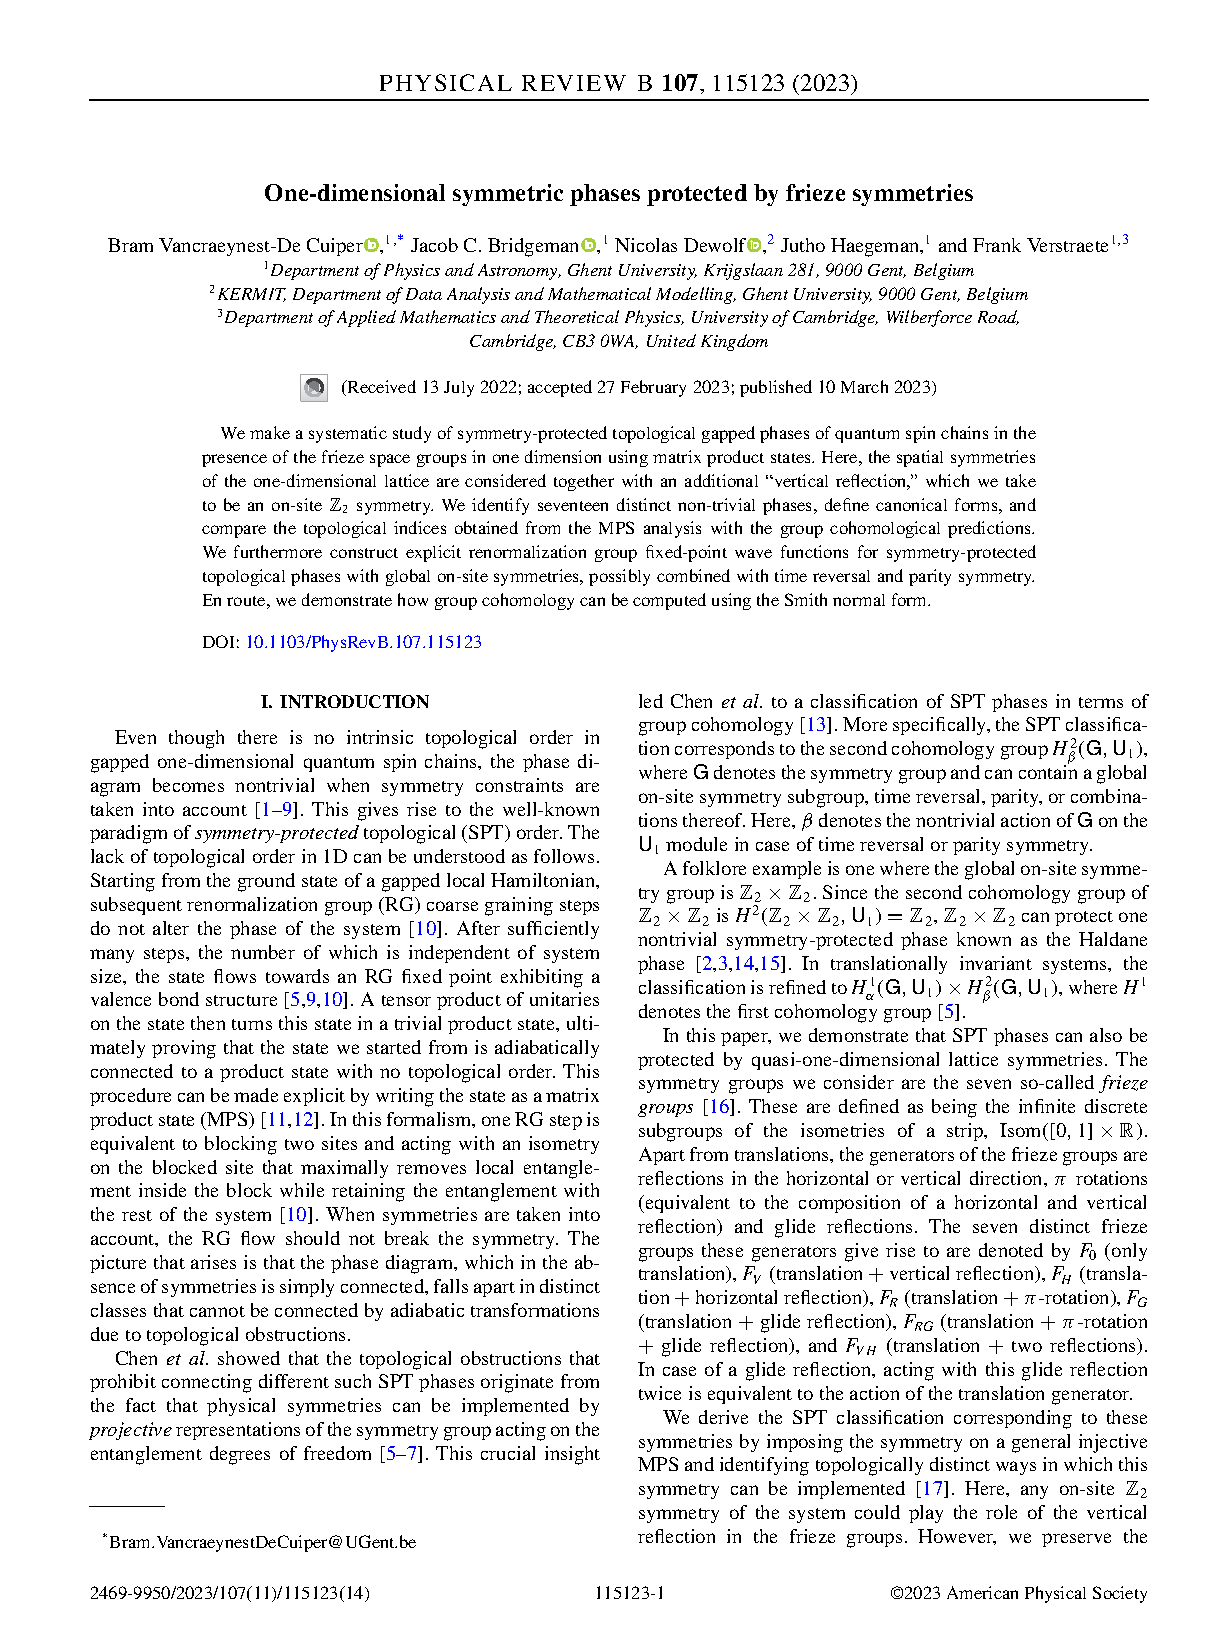
\includepdf[pages=-, trim=0 1.2cm 0 1.2cm, clip=true, frame=false, noautoscale=true, width=1.14\headwidth, offset=-4mm 6mm, , pagecommand={}]{papers/frieze}
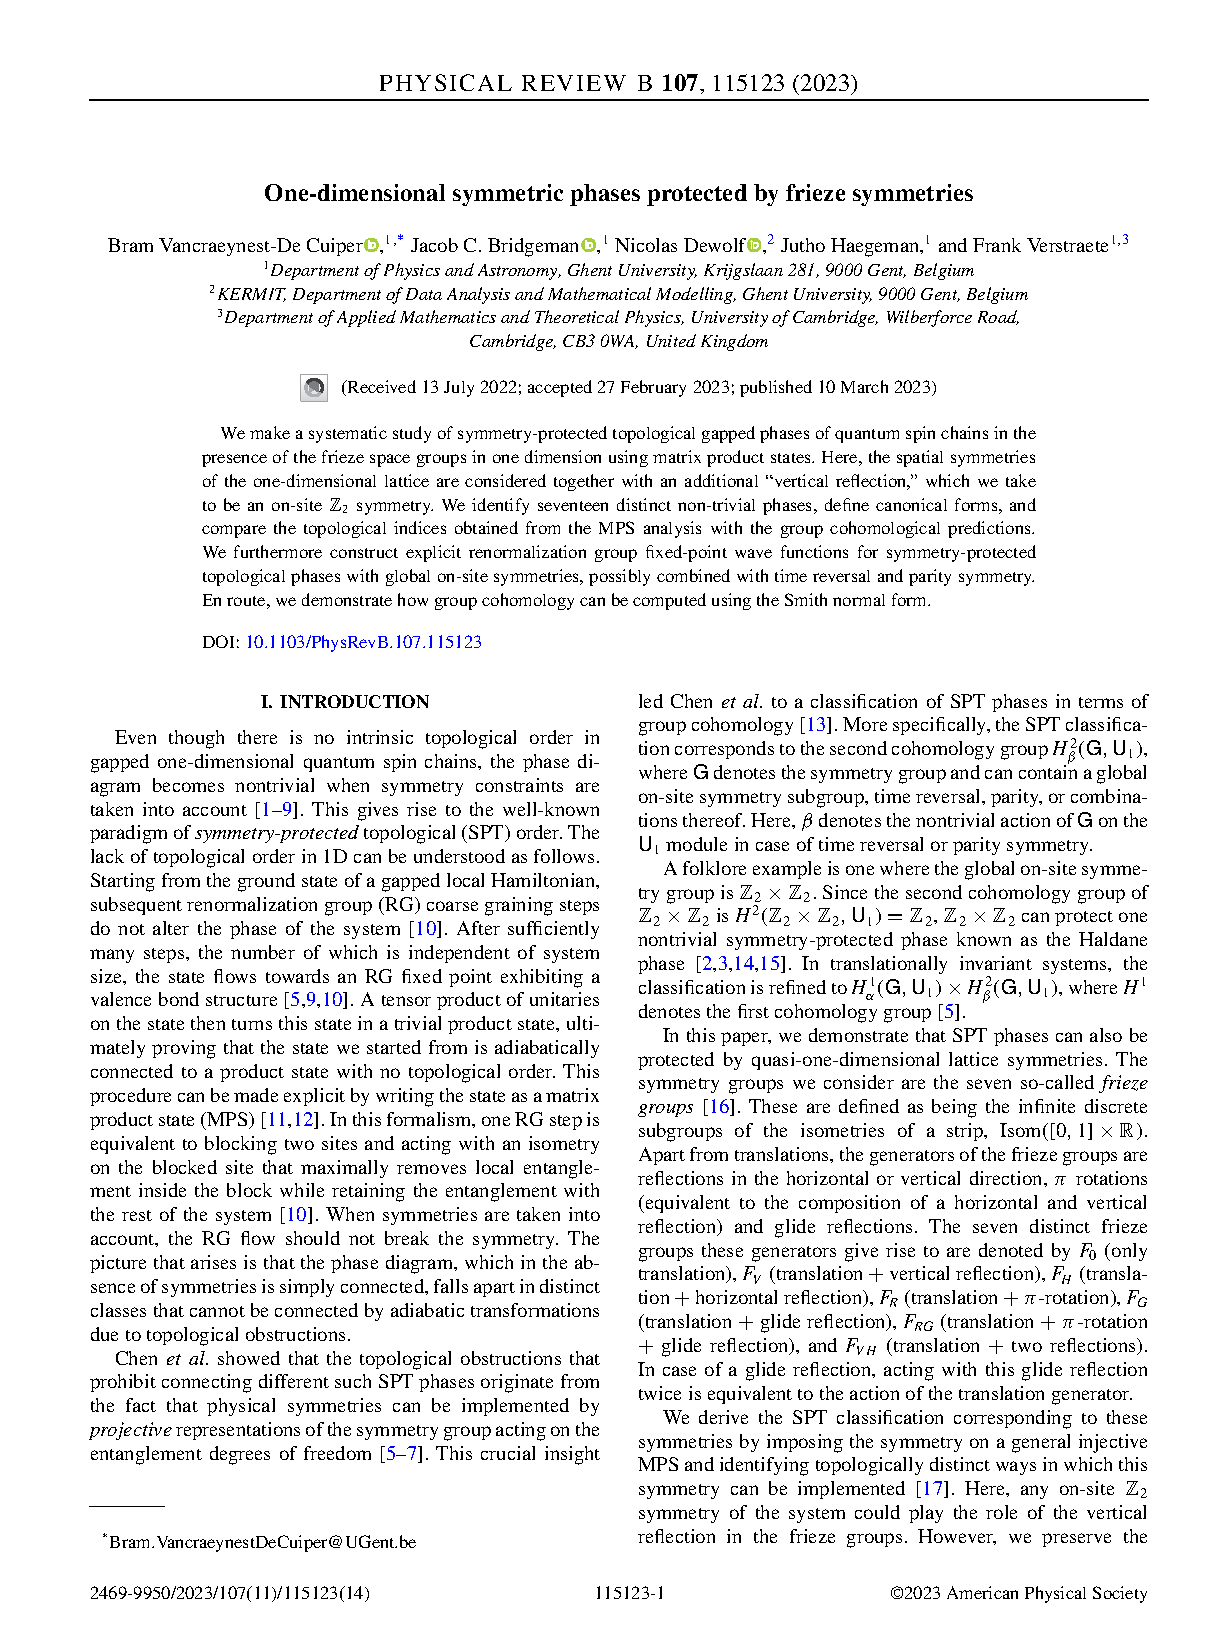
\includepdf[pages=-,
trim=12mm 12.7mm 12mm 9.2mm, clip=true,
noautoscale=true, width=\textwidth,
offset=-0.65mm 5mm,
pagecommand={\thispagestyle{publication}}]{papers/frieze}